% yaml_layers_bw.tex
% Black and white version for Stata Journal
% Classic academic style - no colors, simple borders
% Author: João Pedro Azevedo
% Date: December 2025

\documentclass[tikz,border=10pt]{standalone}
\usepackage{tikz}
\usetikzlibrary{positioning, arrows.meta, fit, backgrounds}

\begin{document}

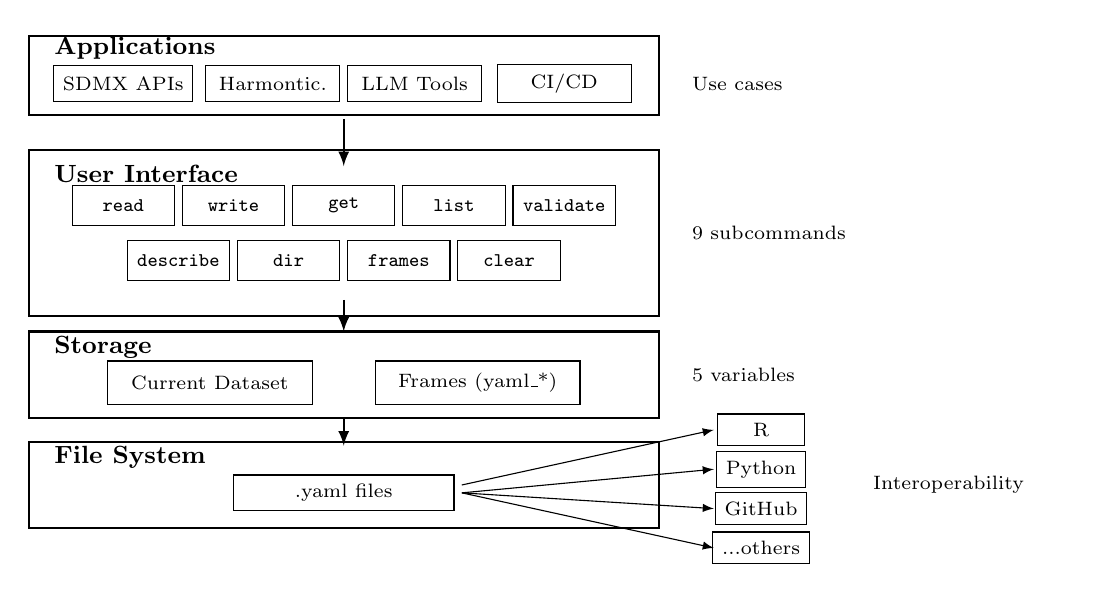
\begin{tikzpicture}[
    % Layer box style - simple black borders
    layer/.style={
        rectangle,
        draw=black,
        thick,
        minimum width=8cm,
        minimum height=1.1cm,
        font=\small
    },
    % Command box style - simple rectangles
    cmdbox/.style={
        rectangle,
        draw=black,
        minimum width=1.3cm,
        minimum height=0.5cm,
        font=\scriptsize\ttfamily
    },
    % Arrow style - simple black
    arrow/.style={
        ->,
        >=latex,
        thick
    },
    % Label style
    lbl/.style={
        font=\small\bfseries
    },
    % Use case box style
    usebox/.style={
        rectangle,
        draw=black,
        minimum width=1.7cm,
        minimum height=0.45cm,
        font=\scriptsize
    }
]

% === Layer 0: Applications / Use Cases (Top) ===
\node[layer, minimum height=1.0cm] (apps) at (0, 5.2) {};
\node[lbl, anchor=west] at (-3.8, 5.55) {Applications};

% Use case boxes
\node[usebox] at (-2.8, 5.1) {SDMX APIs};
\node[usebox] at (-0.9, 5.1) {Harmontic.};
\node[usebox] at (0.9, 5.1) {LLM Tools};
\node[usebox] at (2.8, 5.1) {CI/CD};

% === Layer 1: User Interface ===
\node[layer, minimum height=2.1cm] (ui) at (0, 3.2) {};
\node[lbl, anchor=west] at (-3.8, 3.95) {User Interface};

% Subcommands in UI layer - first row
\node[cmdbox] at (-2.8, 3.55) {read};
\node[cmdbox] at (-1.4, 3.55) {write};
\node[cmdbox] at (0, 3.55) {get};
\node[cmdbox] at (1.4, 3.55) {list};
\node[cmdbox] at (2.8, 3.55) {validate};

% Second row of commands
\node[cmdbox] at (-2.1, 2.85) {describe};
\node[cmdbox] at (-0.7, 2.85) {dir};
\node[cmdbox] at (0.7, 2.85) {frames};
\node[cmdbox] at (2.1, 2.85) {clear};

% === Layer 2: Storage ===
\node[layer] (storage) at (0, 1.4) {};
\node[lbl, anchor=west] at (-3.8, 1.75) {Storage};

\node[rectangle, draw=black, minimum width=2.6cm, minimum height=0.55cm, font=\scriptsize] 
      (dataset) at (-1.7, 1.3) {Current Dataset};
\node[rectangle, draw=black, minimum width=2.6cm, minimum height=0.55cm, font=\scriptsize] 
      (frames) at (1.7, 1.3) {Frames (yaml\_*)};

% === Layer 3: File System ===
\node[layer] (fs) at (0, 0) {};
\node[lbl, anchor=west] at (-3.8, 0.35) {File System};

\node[rectangle, draw=black, minimum width=2.8cm, minimum height=0.45cm, font=\scriptsize] 
      at (0, -0.1) {.yaml files};

% === Other languages (right side of file system) ===
\node[rectangle, draw=black, minimum width=1.1cm, minimum height=0.4cm, font=\scriptsize] 
      (rlang) at (5.3, 0.7) {R};
\node[rectangle, draw=black, minimum width=1.1cm, minimum height=0.4cm, font=\scriptsize] 
      (python) at (5.3, 0.2) {Python};
\node[rectangle, draw=black, minimum width=1.1cm, minimum height=0.4cm, font=\scriptsize] 
      (github) at (5.3, -0.3) {GitHub};
\node[rectangle, draw=black, minimum width=1.1cm, minimum height=0.4cm, font=\scriptsize] 
      (others) at (5.3, -0.8) {...others};

% Arrows from yaml files to other languages
\draw[arrow, thin] (1.5, 0) -- (4.7, 0.7);
\draw[arrow, thin] (1.5, -0.1) -- (4.7, 0.2);
\draw[arrow, thin] (1.5, -0.1) -- (4.7, -0.3);
\draw[arrow, thin] (1.5, -0.1) -- (4.7, -0.8);

% === Arrows between layers ===
\draw[arrow] (0, 4.65) -- (0, 4.05);
\draw[arrow] (0, 2.35) -- (0, 1.95);
\draw[arrow] (0, 0.85) -- (0, 0.5);

% === Side annotations (right margin) ===
\node[font=\scriptsize, anchor=west, text width=2.5cm, align=left] 
    at (4.3, 5.1) {Use cases};
\node[font=\scriptsize, anchor=west, text width=2.5cm, align=left] 
    at (4.3, 3.2) {9 subcommands};
\node[font=\scriptsize, anchor=west, text width=2.5cm, align=left] 
    at (4.3, 1.4) {5 variables};
\node[font=\scriptsize, anchor=west, text width=2.5cm, align=left] 
    at (6.6, 0) {Interoperability};

\end{tikzpicture}

\end{document}
